\section{Theorie}

Der Versuch V602 untersucht das Emissionsspektrum einer $\ce{Cu}-$Röntgenröhre
und Absorptionsspektren verschiedener Absorber.

Röntgenstrahlen werden in einer Röntgenröhre erzeugt. Diese ist
evakuiert und beinhaltet eine Glühkathode und eine Anode.
Aufgrund des Glühelektrischeneffektes werden Elektronen aus der Kathode gelöst und
in Richtung der positiv geladenen Anode beschleunigt. Treffen die beschleunigten
Elektronen auf das Anodenmaterial auf entsteht Röntgenstrahlung, welche sich
aus dem kontinuierlichen Bremsspektrum und der charakteristischen Röntgenstrahlung
zusammensetzt. Die hier auftretende charakteristische Röntgenstrahlung ist
dem Anodenmaterial Kupfer zugeordnet. Das Bremsspektrum wird wegen des
Coulombfeldes des Atomkernes hervorgerufen. Beim Abbremsprozess wird ein Photon
emittiert. Die Energie des Photons entspricht dem Energieverlust des abgebremsten
Elektrons. Die Wellenlänge $\lambda$ des emittierten Photons lässt sich aus der Energie $E\ua{kin}$ über
den folgenden Zusammenhang ermitteln.

\begin{equation}
  \label{eqn:Wellenlänge}
  \lambda = \frac{h\cdot c}{E\ua{kin}}
\end{equation}

Dabei ist $c$ die Lichtgeschwindigkeit und $h$ das \emph{Plank'sche Wirkungsquantum}.
Die Wellenlänge wird minimal für den maximalen Wert der Energie.
Die kinetische Energie ist maximal für $e_0U$, wodurch

\begin{equation}
  \label{eqn:Wellenlänge_minimal}
  \lambda\ua{min} = \frac{h\cdot c}{e_0U}.
\end{equation}

In \eqref{eqn:Wellenlänge_minimal} wird die gesamte kinetische Energie in
Strahlungsenergie umgewandelt.

Das charakteristische Spektrum entsteht aufgrund der Ionisierung des Anodenmaterials.
Dabei wird ein Elektron aus einer inneren Schale herausgelöst.
Die entstandene Leerstelle wird durch ein Elektron der äußeren Schale gefüllt.
Aufgrund der Energiedifferenz der Elektronenschalen wird beim Wechsel eines
äußeren Elektrons auf eine inner liegende Schale ein Röntgenquant mit der
Energie $h\nu = E\ua{m} - E\ua{n}$ emittiert. Die auftretenden Energien $E\ua{m}$
und $E\ua{n}$ stellen die Energien der verschiedenen Elektronenschalen dar.
Das charakteristische Spektrum besteht aus diskreten, scharfen Linien, welche
mit $K_\alpha, K_\beta, L_\alpha, L_\beta, ...$ gekennzeichnet werden. Die
Buchstaben $K, L, M$ stehen dabei für die Elektronenschalen des Atoms und die
Indizes sagen aus, welches Elektron aus der Schale gewechselt ist.
Die Bindungsenergie eines Elektron aus der $n$-ten Schale ist geringer, als
die Bindungsenergie eines Elektrons aus der $n-1$-ten Schale. Dies wird durch
Abschrimungseffekte der Hüllenelektronen und Wechselwirkungen der Elektronen
untereinander welche die Kernladung teilweise kompensieren können verstärkt.
Das charakteristische Spektrum weißt für jedes Elektron spezifische
Linien auf, welche als Feinstruktur bezeichnet werden.
Für die Bindungsenergie $E\ua{n}$ eines Elektron der $n$-ten Schale gilt unter Berücksichtigung der
Feinstruktur nach der Sommerfeldschen Feinstrukturformel:

\begin{equation}
  \label{eqn:Bindungsenergie}
  E\ua{n, j} = -R_\infty\left(z\ua{eff}^2 \cdot \frac{1}{n^2} + \alpha \cdot z\ua{eff}^4 \cdot \frac{1}{n^3}\left(\frac{2}{2j + 1} - \frac{3}{4n}\right)\right).
\end{equation}

Dabei ist $R_\infty = \SI{13,6}{eV}$ die Rydbergenergie, $n$ die Hauptquantenzahl,
$j$ der Gesamtdrehimpuls, $\alpha$ die Sommerfeldsche Feinstrukturkonstante und $z\ua{eff}$
die effektive Kernladung. Diese setzt sich aus der Differenz $z\ua{eff} =  z - \sigma$ zusammen,
wobei $\sigma$ der Abschirmungskonstante ist.

Wird die Feinstruktur vernachlässigt vereinfacht sich die Bindungsenergie eines
Elektrons der $n$-ten Schale zu:

\begin{equation}
  \label{eqn:Bindungsenergie_vereinfacht}
  E\ua{n} = -R_\infty z\ua{eff}^2 \cdot \frac{1}{n^2}.
\end{equation}

Insgesamt spielen bei der Absorption von Strahlung drei grundlegende Effekte
eine Rolle. Zum einen der Photoeffekt, welcher bewirkt, dass einfallende
Photonen Elektronen aus Metalloberflächen lösen können, der Comptoneffekt,
welcher für eine meist unerwünschte Röntgenstrahlenstreuung führt und die Paarbildung.
Paarbildung tritt jedoch nur bei Strahlungsenergien von $>\SI{1}{MeV}$. Diese
werden im vorliegenden Versuch nicht erreicht. Damit sind die
dominant auftretenden Phänomene der Photo- und der Comptoneffekt.
Der Comptoneffekt tritt auf wenn Röntgenstrahlen an den Elektronen des Target
gestreut werden. Die gestreute Röntgenstrahlen besitzen eine längere Wellenlänge
als die eingehende Strahlung. Mit dem Streuwinkel $\theta$ verhält sich der Comptoneffekt gemäß:

\begin{equation}
  \label{eqn:Compton}
  \lambda\ua{einfallend} - \lambda\ua{gestreut} = \frac{h}{m_e\cdot c}\left(1 - \cos \theta\right).
\end{equation}



Die stattfindende Absorption nimmt mit zunehmender Energie der Elektronen ab
und steigt sprunghaft an, sobald die Photonenenergie gerade geößer ist, als
die Bindungsenergie eines Elektrons aus der nächsten tieferen Schale.
Damit ergeben sich die Absorptionskanten zu $h\nu\ua{abs} = E\ua{n} - E\ua{\infty}$.
Die Absorptionskante wird immer nach der Schale aus der das Elektron stammt
als $K$-, $L$-, $M$-,$...$ Kante bezeichnet. In der $L$-Schale lassen sich drei
Absorptionskanten beobachten, wobei aufgrund der Auflösung nur zwei Kanten sichtbar
werden.
Die zugehörige Abschirmungskonstante $\sigma_L$ ergibt sich damit zu:

\begin{equation}
  \label{eqn:sigma_L}
  \sigma_L = Z - \left(\frac{4}{\alpha}\sqrt{\frac{\Delta E_L}{R_\infty}} - \frac{5\Delta E_L}{R_\infty}\right)^{\frac{1}{2}}\left(1 + \frac{19}{32}\alpha^2\frac{\Delta E_L}{R_\infty}\right)^{\frac{1}{2}}.
\end{equation}

In dieser Formel ist $\Delta E_L$ die Energie zwischen der $L_{II}$-- und der $L_{III}$--Kante
und $Z$ die Ordnungszahl.

Die Energie bzw. die Wellenlänge lässt sich mittels der Bragg-Bedingung experimentell
ermitteln. Die in der Röntgenröhre erzeugte Röntgenstrahlung wird auf eine Kristallgitter
Struktur geschossen. Ein Winkel $\Theta$ ist ausgezeichnet als Glanzwinkel.
An diesem Winkel interferieren die Wellenlängen konstruktiv miteinander.
Die Bragg-Bedingung ist gegeben durch:

\begin{equation}
  2d\cdot \sin\left(\Theta\right) = k\cdot \lambda.
  \label{eqn:Winkel}
\end{equation}

Mit der Gitterkonstante $d$ und der gebeugten Wellenlänge $\lambda$.

\section{Durchführung}

Der verwendete Aufbau ist in \ref{fig:Aufbau} dargestellt.

\begin{figure}
  \centering
  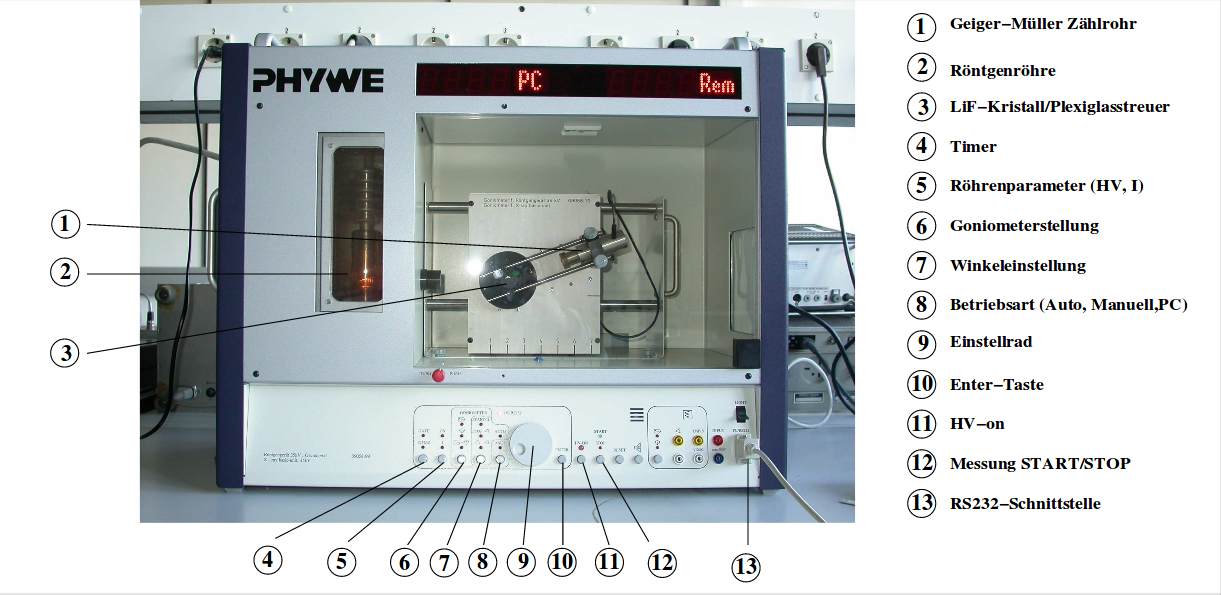
\includegraphics[width=\textwidth]{Pics/Aufbau.png}
  \caption{Aufbau zur Untersuchung der Röntgenemission und -absorption.\cite{anleitung01}}
  \label{fig:Aufbau}
\end{figure}

In der Messapparatur ist im wesentlichen eine Röntgenröhre, ein Geiger-Müller-Zählrohr
mit Drehmechanismus und ein LiF-Kristall integriert. Für die Bedienung der Apparatur und
die Aufnahme der Messdaten wird ein Computer mit vorinstallierter Software verwendet.
Die Beschleunigungsspannung und der Emissionsstrom bleiben während allen Messungen konstant.
$U_B$ liegt bei $\SI{35}{kV}$ und $I$ bei $\SI{1}{\milli\ampere}$.

Zu Begin des Versuches wird die Bragg-Bedingung überprüft.
Dafür wird der Kristallwinkel kostant auf $\Theta = 14°$ eingestellt und das
Geiger-Müller-Zählrohr läuft in einem Winkel von $\alpha_{GM} = 26°$ bis $30°$
mit einem Winkelzuwachs von $\Delta\alpha_{GM}$ um de Kristall herum. Die Integrationszeit
wird auf $\Delta t = \SI{10}{\second}$ eingestellt.

Danach wird das Emissionsspektrum auf das Programm 2:1 Koppelmodus eigestellt.
Das Röntgenspektrum der Beugungsordnung $k = 1$ wird im Winkelbereich
$\Theta = 4°$ bis $26°$ in $0,2°$-Schritten gemessen. Für $\Delta t$
werden $\SI{5}{\second}$ eingestellt.

Abschließend wird das Absorptionsspektrum von fünf leichten Absorbern
und einem schweren Absorber bestimmt. Bei den leichten Absorbern
handelt es sich um $\ce{Zn, Ge, Br, Sr, Zr}$ und bei dem schwerem Absorber handelt
es sich um $\ce{Au}$. Die Braggwinkel zu dem Literaturwert der $E_{K}$-Kante
werden vorher recherchiert, damit $\Theta$ auf $\pm 2°$ des Literaturwertes
eingestellt werden kann. Die Absorber werden vor dem Geiger-Müller-Zählrohr
befestigt. Das Absorptionsspektrum wird in $0,2°$-Schritten mit einer
Integrationszeit von $\Delta t = \SI{20}{\second}$ gestellt.

Alle genommenen Messdaten werden als Grafik und als Tabelle in passendem Format
exportiert.
